\chapter{Methods and Systems Developed}
\label{chapter:Chapter 3}
\lhead{Chapter 3. \emph{Methods and Systems Developed}}

In this Chapter, we present the developed Framework, Firstly by describing the general use of the Modular Framework, Secoundly we provide a detailed explanation of each Module, and his , and i.


\section{Proposed Framework}



\section{Data-Set creation} %This was made for FCD subject, needs much review. 


%\todo[inline]{annotations +  table different sources of data bases}


The initial AIS database was created from a open-source AIS provided by U.S. coastal waters, ~\cite{MarineCadastre}. The raw database file dbf was downloaded, and transformed to a csv, with the use of a open-source GIS software (QGIS). 
 
Before the download of the data-set it was important to select one area of more interest, as dbf to csv transformations are time consuming, and the a decent sized data-set, was achieved with just one area.

\begin{figure}[H]
	\centering
	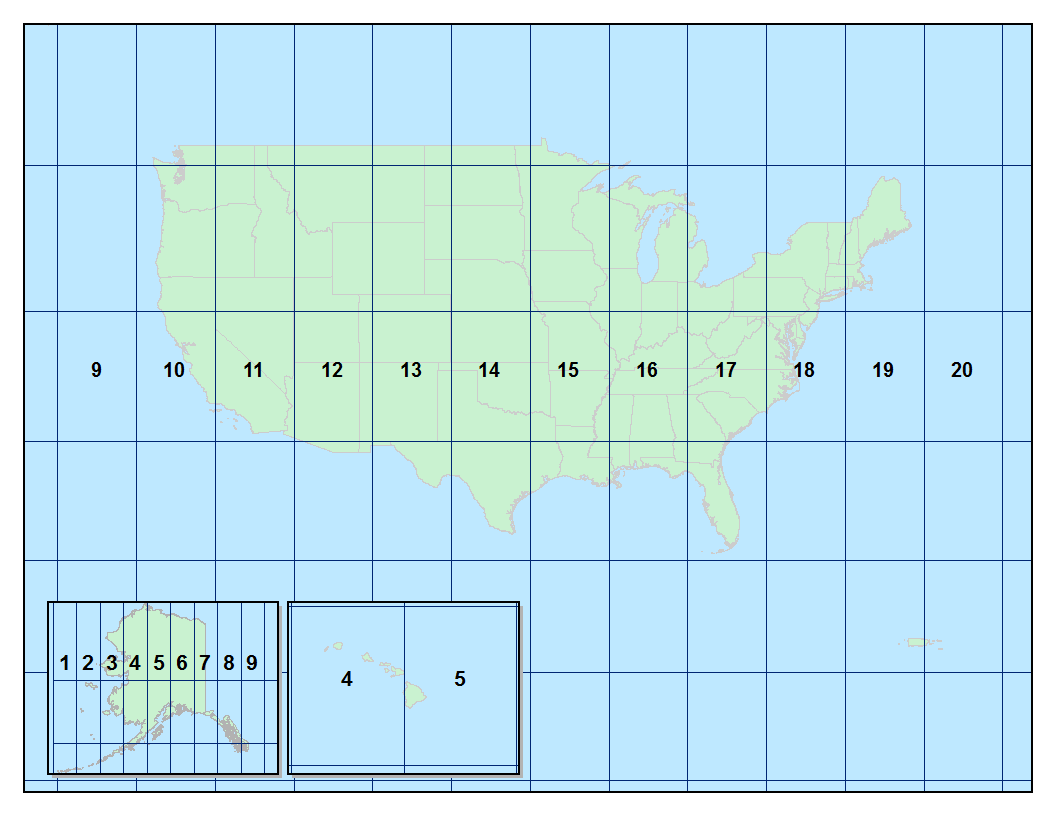
\includegraphics[scale = .35]{figures/UTMZoneMap2014.png}
    \caption{Index map of UTM zones}
    \label{fig: UMT zones}
\end{figure}

The initial selected zone, was zone 10. This zone represents the west coast of the United States, as it is shown in Figure ~\ref{fig: UMT zones}.
The chosen area, represents data whose longitude is from -120 to -126 and latitude is from 30 to 50, from a considerable amount of ships.

%http://www.marinecadastre.gov/ais/

\section{AIS Data}
\label{section: AIS Data}
 With the recent introduction of AIS in the Maritime domain the volume of vessel positional data as exponentially increased, a detailed description of this data, is found in section ~\ref{subsection: chp2_AIS}.

\begin{table}[H]
  \centering
{\small
\begin{tabular}{lrrrrrl}
\toprule
{} &       MMSI &           X &          Y &   SOG &        COG &                Time \\
\midrule
0 &  636081210 & -125.993218 &  48.355773 &  14.3 &  73.300003 & 2014-02-27 13:33:02 \\
1 &  636081210 & -125.985303 &  48.357340 &  14.5 &  73.800003 & 2014-02-27 13:34:23 \\
2 &  636081210 & -125.979437 &  48.358500 &  14.6 &  73.099998 & 2014-02-27 13:35:23 \\
3 &  636081210 & -125.973353 &  48.359692 &  14.7 &  73.000000 & 2014-02-27 13:36:25 \\
4 &  636081210 & -125.965440 &  48.361318 &  15.0 &  73.000000 & 2014-02-27 13:37:46 \\
5 &  636081210 & -125.956733 &  48.363067 &  15.3 &  73.900002 & 2014-02-27 13:39:11 \\
6 &  636081210 & -125.950430 &  48.364153 &  15.7 &  76.099998 & 2014-02-27 13:40:11 \\
7 &  636081210 & -125.944108 &  48.365310 &  15.7 &  74.000000 & 2014-02-27 13:41:10 \\
8 &  636081210 & -125.937763 &  48.366510 &  15.9 &  73.900002 & 2014-02-27 13:42:12 \\
9 &  636081210 & -125.931385 &  48.367660 &  15.9 &  75.000000 & 2014-02-27 13:43:11 \\
\bottomrule
\end{tabular} }
\caption{Example of AIS data transmitted by Vessel, MMSI: 636081210}
\label{Table: TableAIS1}
\end{table}


\section{Route Representation}
Representing the data of a vessel trajectory, can become a difficulty in the Maritime domain. There are a vast number of techniques described in the literature.

A effective way to represent a trajectory in the Maritime domain, is to look to the trajectory as a whole, this is, as vessel are obliged to broadcast their AIS information in a semi-continuous rates; knowing that each AIS broadcast message represent the instantaneous kinematic information from a single vessel, aggregating this information over time will represent a vessel trajectory. Therefore, knowing the MMSI of a vessel, a trajectory can be considered as the set of AIS messages broadcast, by that vessel, identified by the MMSI.


Thus, a possible definition for a vessel trajectory is a, set of multidimensional-points represented as:
\[TR_{MMSI} = p1, p2, p3, p4, \cdots , pn\]

Where each multidimensional point $p$ is defined as:
\[p = [t, x, y, SoG, CoG]\]


%\todo[inline]{ TODO SE FALTAR DADAS A INTERPOLAÇAO REALIZADA}


%for the Representation of MMSI as a track initially, then the assumption... interpolation of missing SOG and COG values. The use of Haversine formula, justify with as vessel motion is linear and no sudden speed exchanges or route exchanges tend to occur in secounds in the marite traffic, so this .

\section{MARISA Requirements}
\subsection{AIS Signal Loss}
Ships equipped with AIS are obliged to keep the AIS autonomously transmitting AIS messages. A way that ships illegally hide their position and possible what the ships is doing objectively, is by switching off the AIS, or finding ways to block the communications of the AIS transmitter with the coastal receivers.

This creates a problem in the maritime domain, has maritime authorities are constantly finding new ways to discover this illegal activities. A method that looks into historical or new streams of data, was developed. 

This method efficiently uses Data Wrangling techniques, in witch with the aid of powerful Python libraries such as Pandas and Data-Frames, the vessels that don't transmit any information for a parametrized time period, are detected and can be reported for maritime authorities for future investigation.

In table ~\ref{Table: AIS signal loss}, results from the above described method are presented, for this work were conducted on a sub-set of the main data-set, that is, from 50 vessel trajectories, which represents 50,000 AIS messages.

\begin{table}[H]
\centering
\caption{Example of the results, obtained for AIS signal loss, with 50 Ships subset.}
\label{Table: AIS signal loss}
\begin{tabular}{@{}lllll@{}}
\toprule
MMSI & X & Y & Time & Signal Loss Time \\ \midrule
316007330 & -125.990797 & 48.867373 & 2014-02-23 21:43:21 & 18 days 13:53:16 \\
316199201 & -123.375432 & 48.430820 & 2014-02-13 12:26:36 & 11 days 08:18:25 \\
338670018 & -121.378175 & 37.977128 & 2014-02-08 20:18:29 & 7 days 20:06:22 \\
367556504 & -122.495912 & 37.869303 & 2014-02-10 20:45:48 & 7 days 01:57:47 \\
... & ... & ... & ... & ... \\
311240050 & -121.781132 & 30.241660 & 2014-02-06 03:15:42 & 0 days 00:18:39 \\
311240012 & -121.725685 & 30.196453 & 2014-02-08 07:34:12 & 0 days 00:08:30 \\ \bottomrule
\end{tabular}
\end{table}

\subsection{Vessel Rendezvous}
A requirement imposed by the MARISA project, was the development of services, able to detect and generate alarms when two or more vessels are approaching close to each other. This in the maritime world can be called as rendezvous.

The concept of rendezvous in the Maritime world is quite complex, as there are numerous legislation. For the purpose of this work, and because the emphasis is on the alarm generation of possible rendezvous, a simplification of this definition is assumed, therefore: 

~\textbf{Vessel Rendezvous}, for this work is considered as the interception or closeness of two or more vessels, in a configurable time period.

An algorithm was developed in which the a distance ~\textbf{d}, is given as a parameter. For every single Vessel Track, the track is partitioned into time-groups(e.g. a time-group of 5min), ~\textbf{t}, defined also as a parameter. If two or more Vessels, are in the same ~\textbf{t} with a distance smaller than ~\textbf{d}, an alarm is generated for those two vessels.

Figure~\ref{fig: VesselRendevouz2d}, shows two different Vessel Routes, with the axis representing the X and Y coordinate, respectively.

\begin{figure}[H]
	\centering
	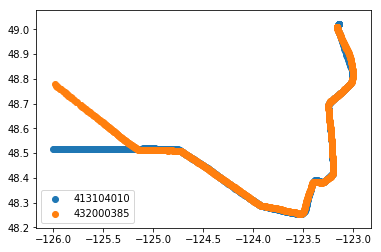
\includegraphics[scale = .8]{figures/VesselRendevouz2d}
    \caption{Two vessel routes}
    \label{fig: VesselRendevouz2d}
\end{figure}

While is obvious that the routes are similar in a positional way, they occur at different times, as is can be see in the figure ~\ref{fig: VesselRendevouz3d} .

\begin{figure}[H]
	\centering
	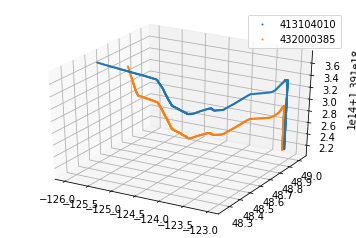
\includegraphics[scale = .9]{figures/VesselRendevouz3d}
    \caption{Two vessel routes, time on Z-axis}
    \label{fig: VesselRendevouz3d}
\end{figure}


   



